\chapter{Исследовательская часть}

\section{Технические характеристики}

Технические характеристики устройства, на котором выполнялось тестирование:
\begin{itemize}
	\item операционная система Ubuntu 22.04.1 LTS Linux x86\_64 \cite{ubuntu};
	\item память 8 ГБ;
	\item процессор Intel® Core™ i3-7130U.
\end{itemize}

Тестирование проводилось на ноутбуке, включенном в сеть электропитания. Во время тестирования ноутбук был нагружен только встроенными приложениями окружения, окружением, а также непосредственно системой тестирования.

\section{Пример работы программы}

На рисунке \ref{img:example} представлен пример работы программы. Вводится размерность первой матрицы и ее элементы, аналогично вводится вторая матрица. Количество столбцов первой матрицы совпадает с количеством строк второй матрицы, значит умножение возможно. Далее выводится результирующая матрица и время выполнения каждого реализованного алгоритма умножения матриц. Все результирующие матрицы совпадают и найдены верно.

\begin{figure}[h]
	\centering
	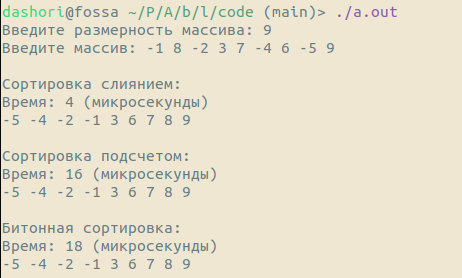
\includegraphics[width=130mm]{images/example}
	\caption{Пример работы программы}
	\label{img:example}
\end{figure}

\clearpage
\section{Время выполнения реализованных алгоритмов}
Замеры времени работы реализованных алгоритмов для квадратных матриц каждой размерности проводились 1000 раз. Каждый раз элементы матриц генерировались случайно -- числа из диапазона~(-INT\_MAX,~INT\_MAX)~\cite{si}. В качестве результата, представленного в таблице~\ref{tab:time}, взято среднее время на каждой размерности матрицы.

\begin{table}[h]
	\begin{center}
		\begin{flushleft}
		\caption{\label{tab:time}Результаты замеров времени реализованных алгоритмов умножения матриц в микросекундах}
		\end{flushleft}
		\begin{tabular}{| l | l | l | l |}
			\hline \specialcell{Размерность\\квадратной матрицы} & \specialcell{Стандартный} &
			\specialcell{Алгоритм\\Винограда} & \specialcell{Оптимизированный\\алгоритм\\Винограда} \\\hline
			2   & 2       & 3       & 3       \\ \hline
			51  & 3662    & 2913    & 2445    \\ \hline
			52  & 3549    & 2792    & 2408    \\ \hline
			101 & 21560   & 16506   & 13810   \\ \hline
			102 & 22220   & 16893   & 14266   \\ \hline
			201 & 167384  & 128039  & 107315  \\ \hline
			202 & 171351  & 131540  & 109524  \\ \hline
			301 & 561385  & 446087  & 371439  \\ \hline
			302 & 588042  & 466535  & 388604  \\ \hline
			401 & 1341353 & 1159066 & 930428  \\ \hline
			402 & 1338481 & 1151987 & 924616  \\ \hline
			501 & 2626258 & 2321114 & 1845890 \\ \hline
			502 & 2625640 & 2311815 & 1828466 \\ \hline
		\end{tabular}
	\end{center}
\end{table}

На рисунке \ref{img:result} представлена зависимость времени работы реализованных алгоритмов умножения матриц, размерность которых является четной. На рисунке \ref{img:resultOdd} представлена зависимость времени работы реализованных алгоритмов умножения матриц, размерность которых является нечетной. 
\begin{figure}[h]
	\centering
	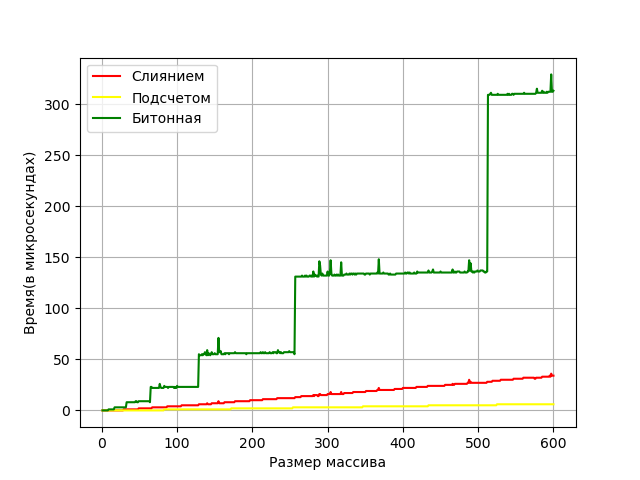
\includegraphics[width=140mm]{images/result}
	\caption{Зависимость времени работы реализованных алгоритмов умножения матриц, размерность которых является четной}
	\label{img:result}
\end{figure}
\begin{figure}[h]
	\centering
	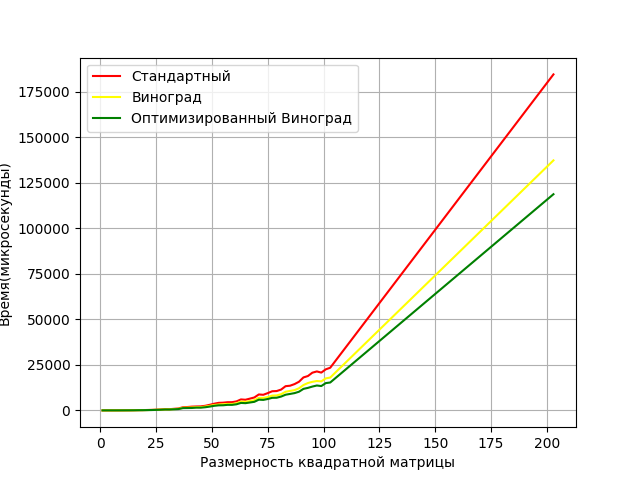
\includegraphics[width=140mm]{images/resultOdd}
	\caption{Зависимость времени работы реализованных алгоритмов умножения матриц, размерность которых является нечетной}
	\label{img:resultOdd}
\end{figure}

\clearpage
Стандартный алгоритм умножения матриц работает дольше, чем алгоритм Винограда и оптимизированный алгоритм Винограда. Например, на рамерах матриц, равных $502$, стандартный алгоритм умножения матриц работает дольше в $1,13$ раз чем алгоритм Винограда и в $1,4$ раз чем оптимизированный алгоритм Винограда.

Также, сравнивая значения времени в таблице \ref{tab:time} можно сделать вывод, что алгоритм Винограда и оптимизированный алгоритм Винограда работают медленнее при нечётных размерах матриц.
